\documentclass[a4paper,12pt]{article}
\usepackage{amsmath,amsfonts,amsthm,amscd,amssymb,latexsym}%,eufrak}
%%%%%%%%%%%%%
\usepackage{caption}
\usepackage{subcaption}
\usepackage{enumerate,graphicx,psfrag}%,subfigure}%,jchangebar,oldgerm}
\usepackage[mathscr]{eucal}
\usepackage[usenames]{color}
\usepackage{url}
\usepackage[shortlabels]{enumitem}
\usepackage{comment}
%\usepackage[utf8]{inputenc}
\usepackage[T1]{fontenc}
%\usepackage{showkeys}
\usepackage{wrapfig}
\usepackage{lscape}
\usepackage{rotating}
%%%%%%%%%
\sloppy
%%%%%%%%%%%%%%%%%%%%%%%
\title{The subgroup membership problem in amalgamated products of 
finitely generated free groups
}
\author{Andrew J. Duncan, Elizaveta Frenkel}

\renewcommand{\a}{\alpha }
\renewcommand{\b}{\beta }
\newcommand{\G}{\Gamma }
\newcommand{\g}{\gamma }
\newcommand{\D}{\Delta }
\renewcommand{\d}{\delta }
%\def\vd{\vardelta}
\newcommand{\ep}{\epsilon }
\newcommand{\e}{\varepsilon }
\newcommand{\z}{\zeta }
%\eta
\renewcommand{\th}{\theta }
\newcommand{\T}{\Theta }
\renewcommand{\i}{\iota }
\renewcommand{\k}{\kappa }
\renewcommand{\l}{\lambda }
\renewcommand{\L}{\Lambda }
%\mu
%\nu
%\xi
%omicron
%\pi
\renewcommand{\r}{\rho }
\newcommand{\s}{\sigma }
\renewcommand{\S}{\Sigma }
\renewcommand{\t}{\tau }
\newcommand{\up}{\upsilon }
\newcommand{\U}{\Upsilon }
%\phi
\newcommand{\x}{\chi }
%\psi
\newcommand{\W}{\Omega }
\newcommand{\w}{\omega }
%%%%%%%%%%%%%%%%%%%%%%%%%%%%%%%
%%%%%%%%%%%%%%%%%%%%%%%%%%%%%
\newcommand{\pd}{\partial}
\newcommand{\wht}{\widehat}
%\newcommand{\cC}{{\mathcal C}}
%\newcommand{\cdim}{\texttt{cdim}}
\newcommand{\fC}{{\textswab C}}
\newenvironment{ef}{\noindent\color{blue} \bf EF: }{}
%
\newcommand{\cA}{{\cal{A}}}
\newcommand{\cD}{{\cal{D}}}
\newcommand{\cF}{{\cal{F}}}
\newcommand{\cH}{{\cal{H}}}
\newcommand{\cJ}{{\cal{J}}}
\newcommand{\cK}{{\cal{K}}}
\newcommand{\cP}{{\cal{P}}}
\newcommand{\cQ}{{\cal{Q}}}
\newcommand{\cR}{{\cal{R}}}
\newcommand{\cS}{{\cal{S}}}
\newcommand{\cV}{{\cal{V}}}
\newcommand{\cW}{{\cal{W}}}
%\newcommand{\GG}{\ensuremath{\mathbb{G}}}
\newcommand{\pp}{\mathbf{p}}
%%%%%%%%%%%%%%%%%%%%%%%%%%%%%%
\newcommand{\nul}{\emptyset }
\newcommand{\vim}{\nu\textrm{-im}}
%%%%%%%%%%%%%%%%%%%%%%%%%%%%%%
\newtheorem{theorem}{Theorem}[section]
\newtheorem{lemma}[theorem]{Lemma}
\newtheorem{corollary}[theorem]{Corollary}
\newtheorem{proposition}[theorem]{Proposition}
\newtheorem{axiom}[theorem]{Axiom}
\newtheorem{definition}[theorem]{Definition}
\newtheorem*{defn*}{Definition}
\newtheorem{conjecture}[theorem]{Conjecture}
%cvs -d :pserver:najd2@cvs.mas.ncl.ac.uk:/CVS/najd2
\newtheorem{exam}[theorem]{Example}
%\newtheorem{comment}[theorem]{Comment}
%
%
\newenvironment{example}{\begin{exam} \rm}{\end{exam}}
%
%
%
\newtheorem{remk}[theorem]{Remark}
\newenvironment{remark}{\begin{remk} \rm}{\end{remk}}
%
%%%%%%%%%%%%
\numberwithin{equation}{section}
\numberwithin{figure}{section}
%%%%%%%%%%%%%%%%%%%%
\newcommand{\Loop}{\operatorname{Loop}}
\newcommand{\Iso}{\operatorname{Isom}}
\newcommand{\Aut}{\operatorname{Aut}}
%%%%%%%%%%%%%%%%%%%
\renewcommand{\AA}{\ensuremath{\mathbb{A}}}
\newcommand{\ZZ}{\ensuremath{\mathbb{Z}}}
\newcommand{\QQ}{\ensuremath{\mathbb{Q}}}
\newcommand{\RR}{\ensuremath{\mathbb{R}}}
\newcommand{\NN}{\ensuremath{\mathbb{N}}}
\newcommand{\CC}{\ensuremath{\mathbb{C}}}
\newcommand{\FF}{\ensuremath{\mathbb{F}}}
%\renewcommand{\ker}{\verb"Ker"}
\newcommand{\cC}{\mathcal{C}}
\renewcommand{\cF}{\mathcal{F}}
\newcommand{\cO}{\mathcal{O}}
\renewcommand{\cS}{\mathcal{S}}
\newcommand{\la}{\langle}
\newcommand{\ra}{\rangle}
%\newcommand{\BA}{\ensuremath{\mathbb{A}}}
%%%%%%%%%%%%%%%%%%%%%%%%%%%%%%%%%%%%%%
\newcommand{\maps}{\rightarrow}
\newcommand{\ov}[1]{\overline{#1}}
\newcommand{\bs}{\backslash}
%%%%%%%%%%%%%%%%%%%%%%%%%%%%%%%
\newcommand{\be}{\begin{enumerate}}
\newcommand{\ee}{\end{enumerate}}
\newcommand{\bd}{\begin{description}}
\newcommand{\ed}{\end{description}}
\newcommand{\biz}{\begin{itemize}}
\newcommand{\eiz}{\end{itemize}}
%%%%%%%%%%%%%%%%%%%%%%%%%%%%%%%%%%%
%
\newenvironment{ajd1}{\noindent\color{red} AJD }{}
\newcommand{\ajd}[1]{\begin{ajd1} #1 \end{ajd1}}
%
%\includecomment{comp}% to see environment comp
\excludecomment{comp}% to hide environment comp
%
\begin{document}
$F_1=F( x_1,x_2)$, $F_2=F(y_1, y_2)$, $H_1=\la x_2x_1^{-1}, x_2^3, x_2x_1x_2,
x_1^{-1}x_2\ra$, $H_2$ is the same with $y_1$ instead of $x_1$ and $y_2$ instead
of $x_2$. $\phi_1$ maps $z_1$ to $  x_2x_1^{-1}$, $z_2$ to $x_2^3$, $z_3$ to 
 $x_2x_1x_2$ and $z_4$ to $x_1^{-1}x_2$. $\phi_2$ does the same but 
with $y_i$ in place of $x_i$. $H_k$ is normal in $F_k$.
The Stallings folding for $H_1$ is shown in figure \ref{fig:fold}.
\begin{figure}
\begin{center}
\psfrag{a1}{$x_1|z_1^{-1}$}
\psfrag{a2}{$x_1|z_3$}
\psfrag{a3}{$x_1|z_4^{-1}$}
\psfrag{b1}{$x_2|1$}
\psfrag{b2}{$x_2|z_2$}
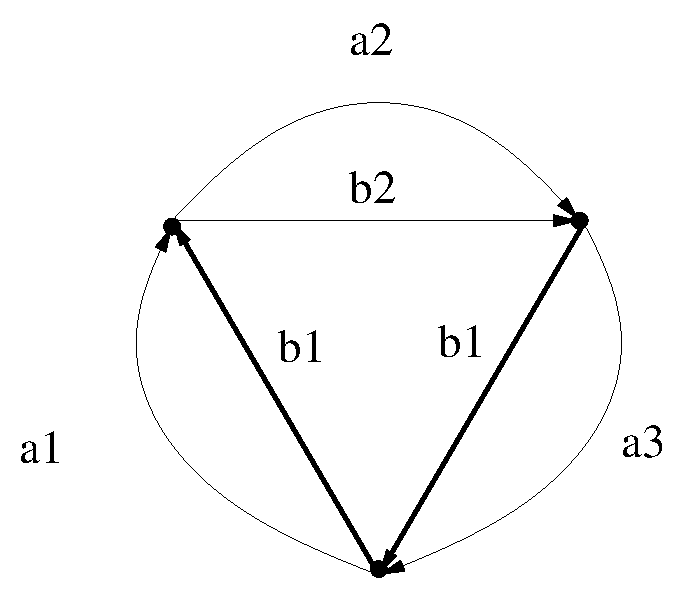
\includegraphics[scale=0.6]{ce.eps}
\caption{}\label{fig:fold}
\end{center}
\end{figure}
\\[1em]

\par\noindent $K=\la y_1x_1,x_1^{-1}x_2\ra$. \\[1em]
$K\cap H_1$ contains $y_1x_1$ and, for all $n>0$, $K$ contains
\begin{align*}
(y_1x_1)^{-n}(x_1^{-1}x_2)(y_1x_1)^{n}&=(y_1x_1)^{(1-n)}x_1^{-1}[y_1^{-1}(y_1^{-1}y_2)y_1]x_1(y_1x_1)^{(n-1)},\\
&=(y_1x_1)^{(1-n)}x_1^{-1}[x_1^{-1}(x_1^{-1}x_2)x_1]x_1(y_1x_1)^{(n-1)},\\
&=(y_1x_1)^{(1-n)}x_1^{-2}(x_1^{-1}x_2)x_1^2(y_1x_1)^{(n-1)},\\
&\vdots\\
&=x_1^{-2n}(x_1^{-1}x_2) x_1^{2n},
\end{align*}
and similarly
\[(y_1x_1)^{n}(x_1^{-1}x_2)(y_1x_1)^{-n}=x_1^{2n-1}(x_2x_1^{-1}) x_1^{-(2n-1)},\]
 using the fact that $H_i$ is normal. 
As $H_1$ is normal both of these are in fact in $K\cap H_1$. \\[1em]
Therefore, for all $n\in \ZZ$, $K\cap H_1$ contains $x_1^{-2n}(x_1^{-1}x_2) x_1^{2n}$. \\[1em]
Let $L=\la x_1^{-2n}(x_1^{-1}x_2) x_1^{2n}|n\in \ZZ\ra\le K$. Then (by induction)  
\[L=\{x_1^{2n_1}(x_1^{-1}x_2)^{r_1}x_1^{2n_2}\cdots (x_1^{-1}x_2)^{r_k}x_1^{2n_{k+1}}\,|\,n_i,r_i\in\ZZ, \sum n_i=0\},\]
$K=\la L, y_1x_1\ra$ 
and also $L$ is normal in $K$, as $(y_1x_1)^{-\e}(x_1^{-2n}(x_1^{-1}x_2) x_1^{2n})(y_1x_1)^{\e}\in L$.  
The subgroup $\la y_1x_1\ra$ consists of elements with reduced (amalgam) form $(y_1x_1)^n$ and none 
of these belong to a factor, except when $n=0$, so $L\cap \la y_1x_1\ra=\{1\}$. 
Therefore
$K=L\rtimes \la y_1x_1\ra$, the internal semi-direct product of $L$ and $\la y_1x_1\ra$. 
Figure \ref{fig:Kfold_inf} shows a folded automaton, based at $1$, which accepts  $K$.
 An arbitrary element of $K$ has the form $l(y_1x_1)^r$, where $l\in L$, $r\in\ZZ$, and reduced forms of 
 elements of the form $l(y_1x_1)^r$ can be read off this diagram.  
It follows that 
 the intersection of $K$ and $H_1$ is $L$ and  representatives for all 
elements of $L$ are required. 
 If $y_1$ is deleted from Figure \ref{fig:Kfold_inf} 
 then a  Stallings folding for the subgroup $L$ of $F_1$ is left, so $L$ has infinite
rank in $F_1$. This means infinitely many representatives (of whatever kind are used) 
 for elements of $L$ will 
be needed. 
\begin{figure}
\begin{center}
\psfrag{x1}{$x_1$}
\psfrag{x2}{$x_2$}
\psfrag{y1}{$y_1$}
\psfrag{1}{$1$}
\includegraphics[scale=0.3]{Kfold_inf.eps}
\caption{}\label{fig:Kfold_inf}
\end{center}
\end{figure}
%\bibliographystyle{plain}
%\bibliography{membership}

Here $H_1$ intersects with infinitely many conjugates of $x_1^{-1}x_2$ which lie in $K$, but
the conjugating elements are not elements of $K$ (they are all of the form $x_1^{2n}$), so 
$K$ is not malnormal. 
(By way of contrast, if, instead of 
$y_1x_1$ we had $x_1^2$ as the 2nd generator of $K$, then the $y_1$ arrow would become an $x_1$ 
above, and the diagram above would collapse to the middle three arrows, to the left of $1$.
All conjugating elements would be in $K$; but of course $K\le H_1$.)

%elements in $K$ again, but in this case the conjugators would belong to $K$.) 
The conjugates of  $x_1^{-1}x_2$ in $K$ are generated by the process of rewriting $H_1$ to $H_2$ then
$H_2$ to $H_1$, as many times as necessary. 
This example is constructed to make this happen in the most obvious way, but
there are probably many less obvious ways in which this may occur.

The membership problem should be solvable in this example: a good algorithm to produce
an acceptor for normal forms for $K$ should give something like the diagram above; in terms of $z$'s. 
Using the periodicity of the diagram the MP is then solvable (I haven't checked carefully).
 
\end{document}

